\documentclass[a4paper, 11pt, french]{article}
\usepackage[utf8]{inputenc}
\usepackage[T1]{fontenc}
\usepackage{babel}
\usepackage{hyperref}
\hypersetup{colorlinks=true, linkcolor=black}
\usepackage{enumitem}
\usepackage{numprint}
\usepackage{parskip}
\usepackage[margin=2.5cm]{geometry}
\usepackage{minted}
\usemintedstyle{vs}
\usepackage{graphicx}
\usepackage{wrapfig}
\usepackage{tikz}
\usepackage[framemethod=TikZ]{mdframed}
\usepackage{listings}
\usepackage{subcaption}

\title{Simulation Orientée-Objet de systèmes multiagents}
\author{}
\date{}

\begin{document}

\maketitle

\section{Choix de conception et tests}

\subsection{Balles}

On a créé une classe \verb|Balls| qui contient la liste des balles (stockée sous forme de points) ainsi que leurs positions initiales. On a écrit des méthodes classiques sur \verb|Balls| comme par exemple accéder au nombre de balles, définir les coordonnées des balles, mais aussi une méthode \verb|transaction|, et \verb|reInit| qui replace les balles à leurs positions initiales.

Ensuite, on a testé notre classe en prenant 3 balles et en essayant de les translater. On a évidemment aussi essayé, une fois déplacées, de replacer les balles à leurs positions initiales. On obtient le résultat suivant.

\begin{verbatim}
[java.awt.Point[x=0,y=0], java.awt.Point[x=3,y=2], java.awt.Point[x=5,y=0]]
[java.awt.Point[x=-1,y=7], java.awt.Point[x=2,y=9], java.awt.Point[x=4,y=7]]
[java.awt.Point[x=0,y=0], java.awt.Point[x=3,y=2], java.awt.Point[x=5,y=0]]
\end{verbatim}

\subsection{Simulateur de balles}

Pour cette classe qui implémente \verb|Simulable|, on a définit comme attribut \verb|balls|, de type \verb|Balls|, qui contient donc les positions actuelles et initiales des balles. On a aussi comme attribut la liste \verb|dir| des vecteurs vitesses de ces balles, ainsi que \verb|dir_init| qui correspond aux vitesses initiales.

Ainsi, quand on va replacer les balles au centre, on va bien pouvoir à la fois les remettre à leurs positions initiales tout en ayant les mêmes vitesses initiales. On ajoute aussi \verb|window| de type \verb|GUISimulator| pour pouvoir dessiner. On ajoute \verb|width|, \verb|height| et \verb|colors| car on les utilise dans notre algorithme même s'ils ne semblent pas indispensables mais cela facilite notre algorithme.

On définit ensuite comme demandé les méthodes \verb|next| et \verb|restart| en faisant bien attention de bien recalculer les nouvelles positions et vitesses des balles et on fait aussi attention à bien \textit{reset} \verb|window| avant de redessiner.

Ensuite, on teste notre classe en créant 6 balles et on lance la simulation.

\begin{figure}[H]
    \centering
    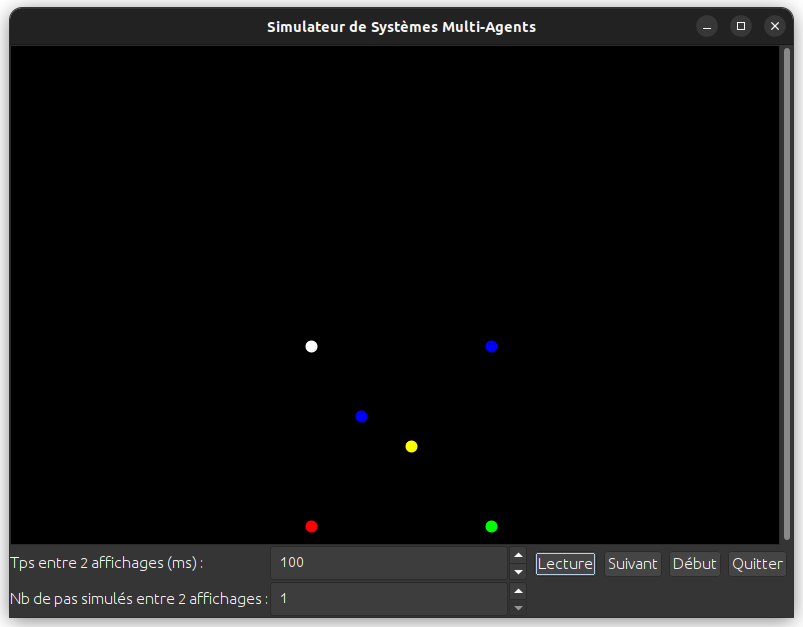
\includegraphics[width=0.38\textwidth]{TestBallsSimulator.png}
    \caption{Résultat de la simulation de \texttt{TestBallsSimulator}}
\end{figure}

\subsection{Jeu de la vie de Conway}

On crée tout d'abord une classe \verb|Cellule| qui nous donne le nombre d'états possibles de la cellule en question et son état actuel. On le fait car on voit que, dans le prochain jeu, on aura besoin de plusieurs états et non seulement deux comme ici puisque la cellule ne peut être que vivante ou morte.

Ensuite, on crée notre classe \verb|Grille| qui implémente \verb|Simulable| et qui va stocker la grille en cours et la prochaine. Cela nous permet, lors du calcul de la prochaine grille, de bien tenir compte des anciennes cellules, et qu'on ne prenne donc pas en compte une nouvelle. Cela n'aurait pas été possible si l'on écrasait directement la valeur. On stocke aussi la grille initiale, histoire de pouvoir revenir au cas initial. Enfin, on a aussi les tailles \verb|n|, \verb|m| et \verb|window| en attribut (pour pouvoir dessiner toujours).

On y définit aussi les méthodes \verb|dessiner|, \verb|next| et \verb|restart|. \verb|dessiner| et \verb|next| sont en \verb|abstract| car on va les écrire spécifiquement en fonction du jeu (\verb|Conway| ou \verb|Immigration|).

Dans le cas du jeu \verb|Conway|, on étend la classe \verb|Grille| en écrivant \verb|dessiner|. Pour cela, on parcourt toute la grille et on change juste la couleur du rectangle affiché en fonction de l'état de la cellule (morte ou vivant). Pour la méthode \verb|next|, on parcourt aussi toute la grille mais on fait bien attention à placer la nouvelle valeur calculée dans \verb|grilleApres|, histoire que \verb|grilleAvant| ne soit pas modifiée lors du calcul. On raisonne par \verb|modulo| pour traiter le cas des bords. Ce n'est qu'à la fin de tous les calculs qu'on va recopier la \verb|grilleApres| dans la \verb|grilleAvant| : dans notre cas, on le fait au tout début de la fonction \verb|dessiner|.

On teste ainsi notre classe avec une grille de taille $10 \times 10$.

\begin{figure}[H]
\centering
\begin{subfigure}{0.3\textwidth}
    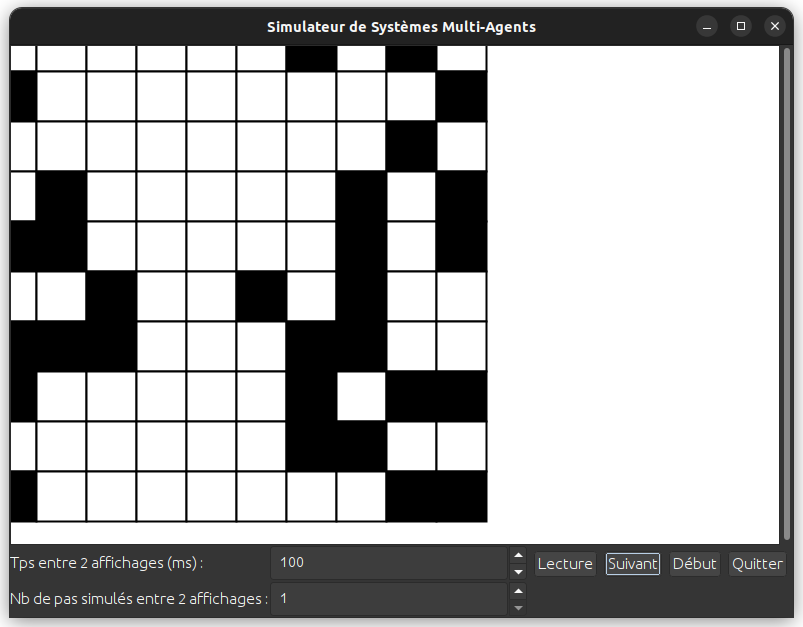
\includegraphics[width=\textwidth]{TestConway1.png}
\end{subfigure}
\hfill
\begin{subfigure}{0.3\textwidth}
    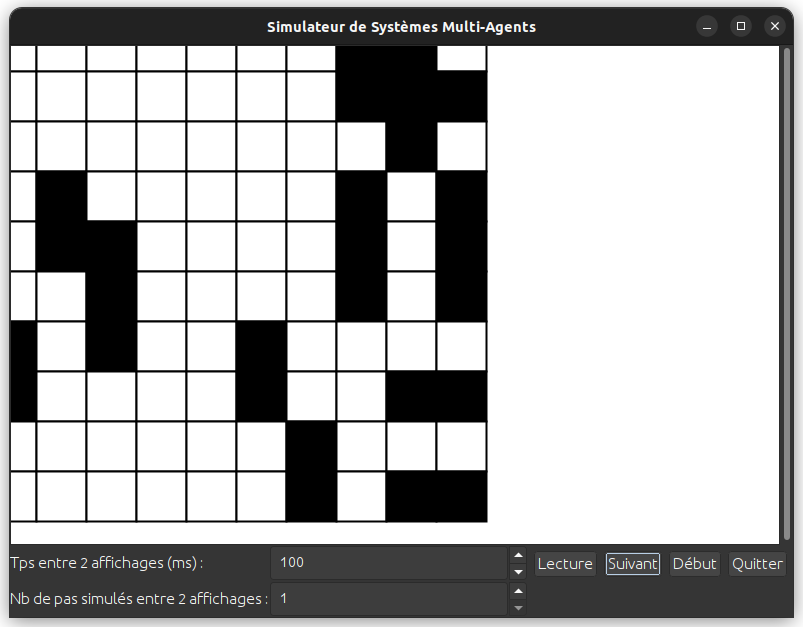
\includegraphics[width=\textwidth]{TestConway2.png}
\end{subfigure}
\hfill
\begin{subfigure}{0.3\textwidth}
    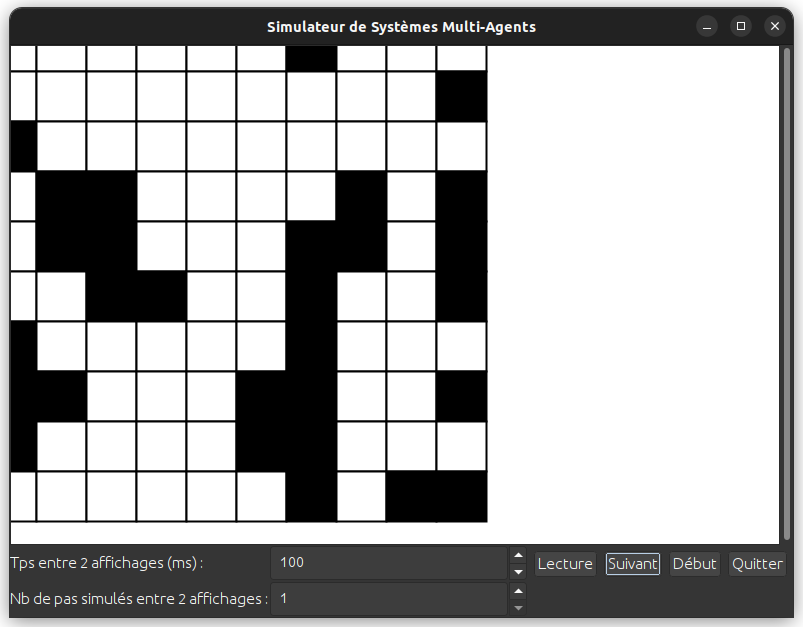
\includegraphics[width=\textwidth]{TestConway3.png}
\end{subfigure}
\caption{Résultat de la simulation de \texttt{TestConway} avec 3 états consécutifs}
\end{figure}

\subsection{Jeu de l'immigration}

C'est exactement le même principe que précédemment sauf qu'au lieu d'avoir seulement 2 états par cellule, on en a $n$. Le seul changement est qu'on stocke le nombre d'états car on l'utilise dans la méthode \verb|next|.

On teste aussi notre classe avec une grille de taille $15 \times 10$, chaque cellule pouvant avoir 5 états.

\begin{figure}[H]
\centering
\begin{subfigure}{0.3\textwidth}
    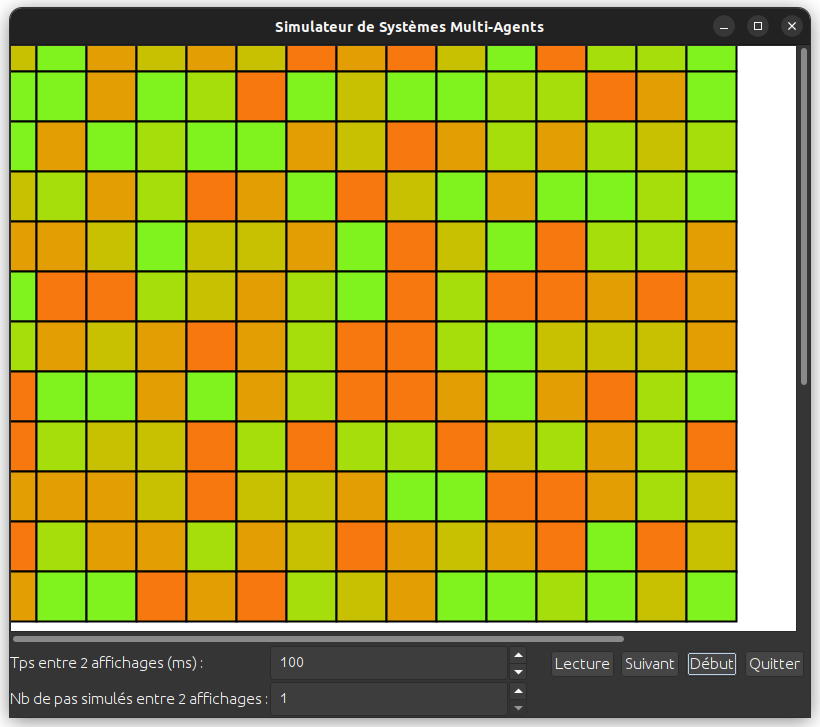
\includegraphics[width=\textwidth]{TestImmigration1.png}
\end{subfigure}
\hfill
\begin{subfigure}{0.3\textwidth}
    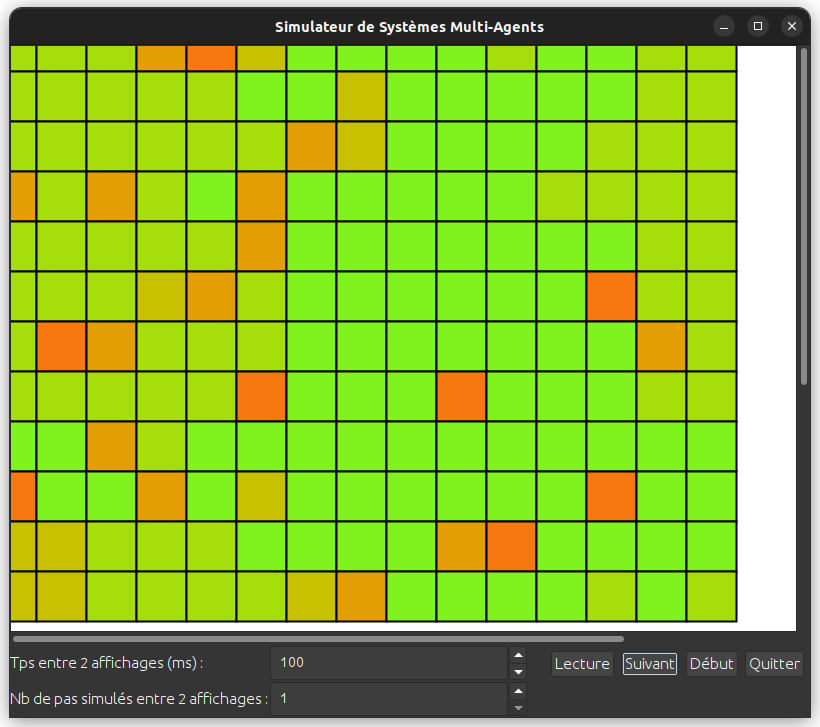
\includegraphics[width=\textwidth]{TestImmigration2.png}
\end{subfigure}
\hfill
\begin{subfigure}{0.3\textwidth}
    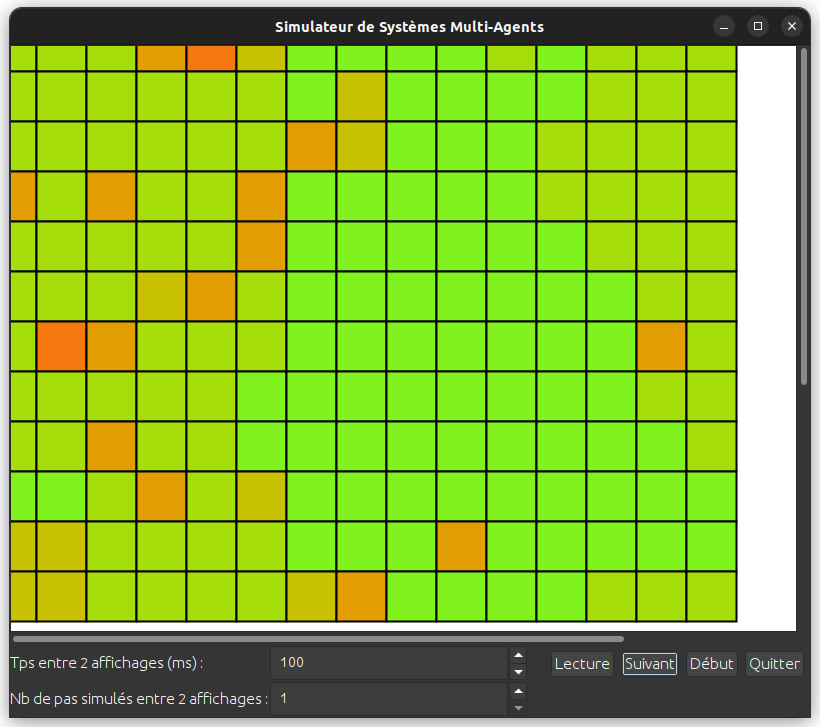
\includegraphics[width=\textwidth]{TestImmigration3.png}
\end{subfigure}
\caption{Résultat de la simulation de \texttt{TestImmigration} avec 3 états consécutifs}
\end{figure}

\subsection{Modèle de Schelling}

Cette classe est, comme précédemment, une extension d'une grille, sauf qu'on ajoute comme attribut une file qui contient l'ensemble des habitations vacantes. On a aussi besoin d'une file temporaire \verb|tmp|. En effet, lorsqu'on va calculer la prochaine file d'habitations vacantes, on a besoin de stocker dans \verb|tmp| les habitations qui ont été quittées, et qui donc sont devenues libres.

On considère qu'une habitation laissée libre ne peut pas directement être habitée, on doit attendre un tour pour qu'elle puisse se remplir à nouveau (après un \verb|next| donc). Ainsi, les habitations qui vont être quittées vont être mises dans \verb|tmp| pour ne pas qu'elle puisse être habitées directement (ce qui aurait été le cas si on la mettait dans la file des habitations vacantes). On va bien évidemment supprimer une habitation vacante de la file pour que la nouvelle habitation puisse y habiter. Ce n'est qu'à la toute fin, qu'on va remettre tous les éléments de \verb|tmp| dans la file des habitations vacantes pour qu'elles puissent être habitées à partir du prochain tour.

Lors de notre calcul pour savoir si une habitation va déménager ou non, on a besoin de compter le nombre de couleurs différentes (sans les doublons évidemment), donc on choisit la collection \verb|Set| (pour qu'on puisse manipuler des ensembles). On précise aussi, que s'il y a $n$ couleurs, il y aura $n+1$ états (0 pour une habitation non habitée, et enfin de 1 à $n$ pour les $n$ couleurs).

On teste notre classe avec 6 états (3 couleurs, et habitation vide) et $K=3$ (seuil).

\begin{figure}[H]
\centering
\begin{subfigure}{0.3\textwidth}
    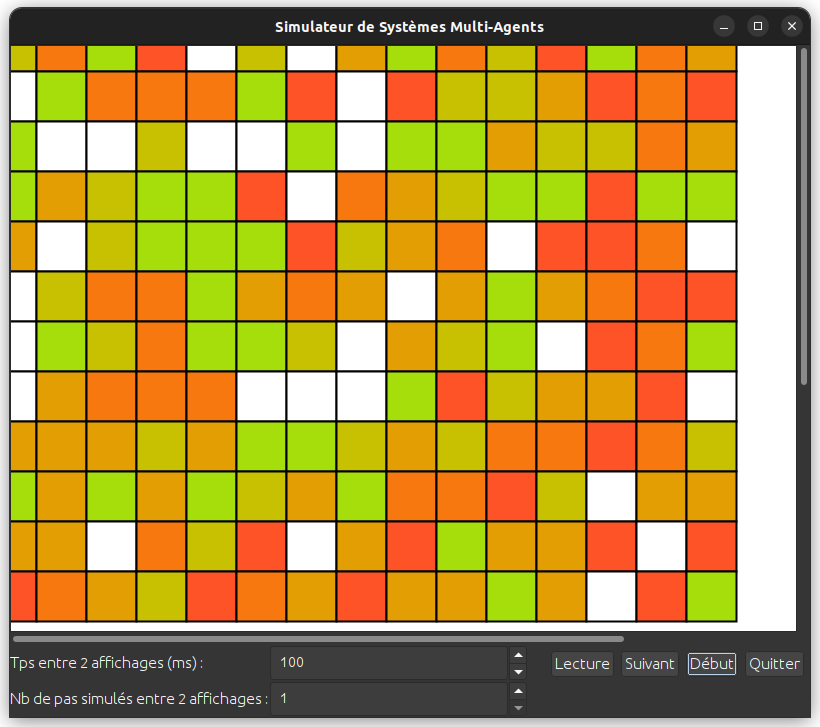
\includegraphics[width=\textwidth]{TestSchelling1.png}
\end{subfigure}
\hfill
\begin{subfigure}{0.3\textwidth}
    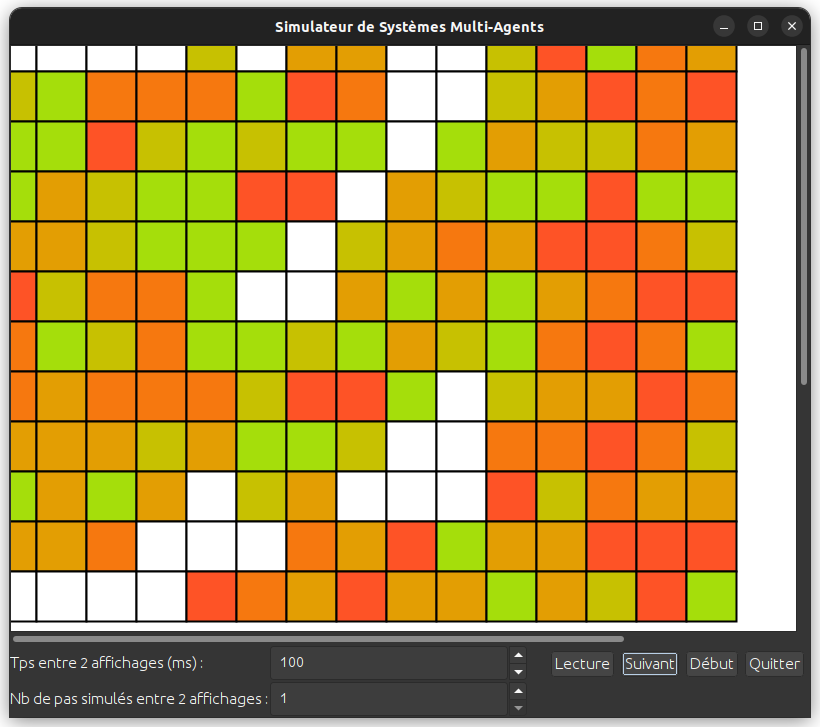
\includegraphics[width=\textwidth]{TestSchelling2.png}
\end{subfigure}
\hfill
\begin{subfigure}{0.3\textwidth}
    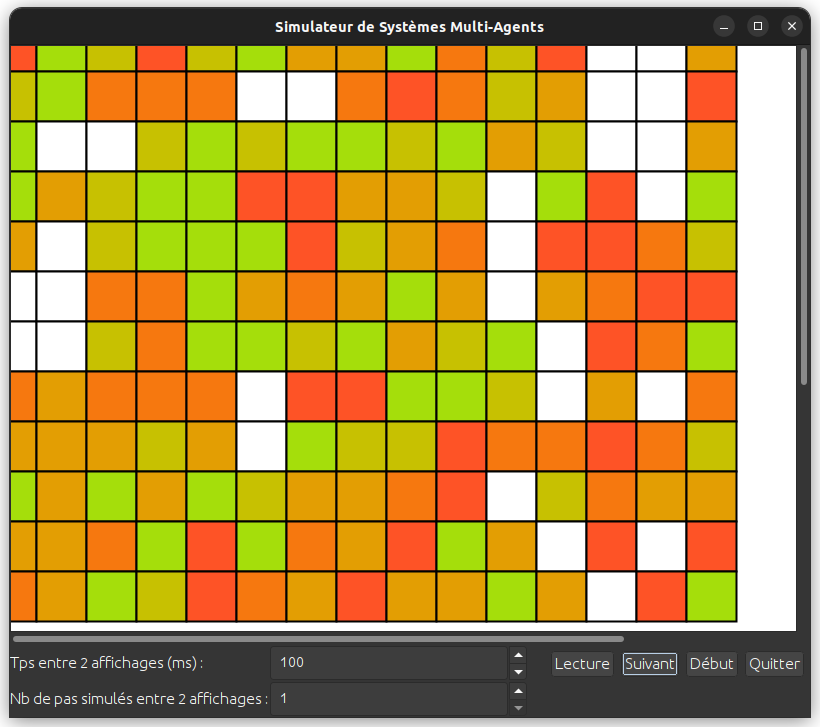
\includegraphics[width=\textwidth]{TestSchelling3.png}
\end{subfigure}
\caption{Résultat de la simulation de \texttt{TestSchelling} avec 3 états consécutifs}
\end{figure}

\subsection{Boids}

On crée une classe \verb|Boid| qui va représenter un essaim avec ses coordonnées, ainsi que son vecteur vitesse. On écrit les fonctions classiques qui permettent d'accéder et de modifier les attributs privés. On réécrit aussi la méthode \verb|equals| de la classe \verb|Object| car on va l'utiliser plus tard.

Ensuite, on crée la classe \verb|BoidsSimulator| avec comme attributs principaux la liste de boids actuelle, la liste de boids à l'état initial, ainsi que \verb|window| pour pouvoir dessiner. On rajoute aussi \verb|height|, \verb|width| et \verb|nb| (nombre de boids) pour faciliter notre code. 

Pour cette classe, on code les 3 règles classiques : cohésion, séparation et alignement. On rajoute aussi la règle \verb|bound_position| pour éviter que les essaims sortent de l'écran. Comme notre classe hérite de l'interface \verb|Simulable|, on réécrit également les méthodes \verb|next| et \verb|restart|. On rajoute aussi une méthode pour dessiner.

Pour dessiner, on créé une classe \verb|Triangle| qui implémente \verb|GraphicalElement| et qui permet à partir des coordonnées (\verb|x| et \verb|y|) ainsi que du vecteur vitesse (\verb|velX| et \verb|velY|) de dessiner l'essaim. Pour cela, on recode la fonction \verb|paint| de \verb|GraphicalElement|.

Enfin, on teste notre simulation avec 100 essaims, \verb|height = 500| et \verb|width = 500|. On précise aussi que initialement, on prend comme vecteur vitesse le vecteur de coordonnées (50, -50). Pour ce qui est des coordonnées initiales, on les choisit aléatoirement en faisant bien attention à ce qu'ils soient dans l'écran.

\begin{figure}[H]
    \centering
    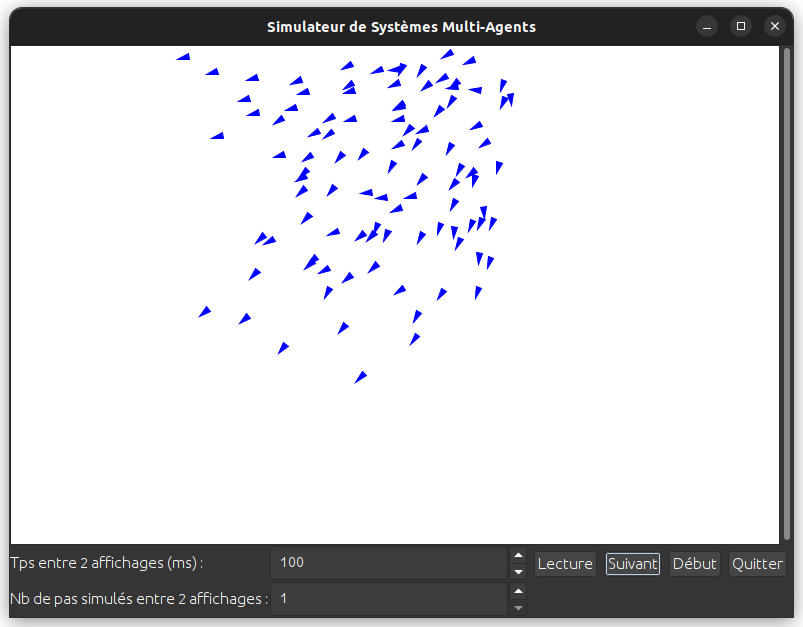
\includegraphics[width=0.7\textwidth]{TestBoidsSimulator.png}
    \caption{Résultat de la simulation de \texttt{TestBoidsSimulator}}
\end{figure}

\newpage

\section{Diagrammes de classes}

Les diagrammes des classes implémentées sont présentés en figures~\ref{fig:graph1} et \ref{fig:graph2}.

\begin{figure}[H]
    \centering
    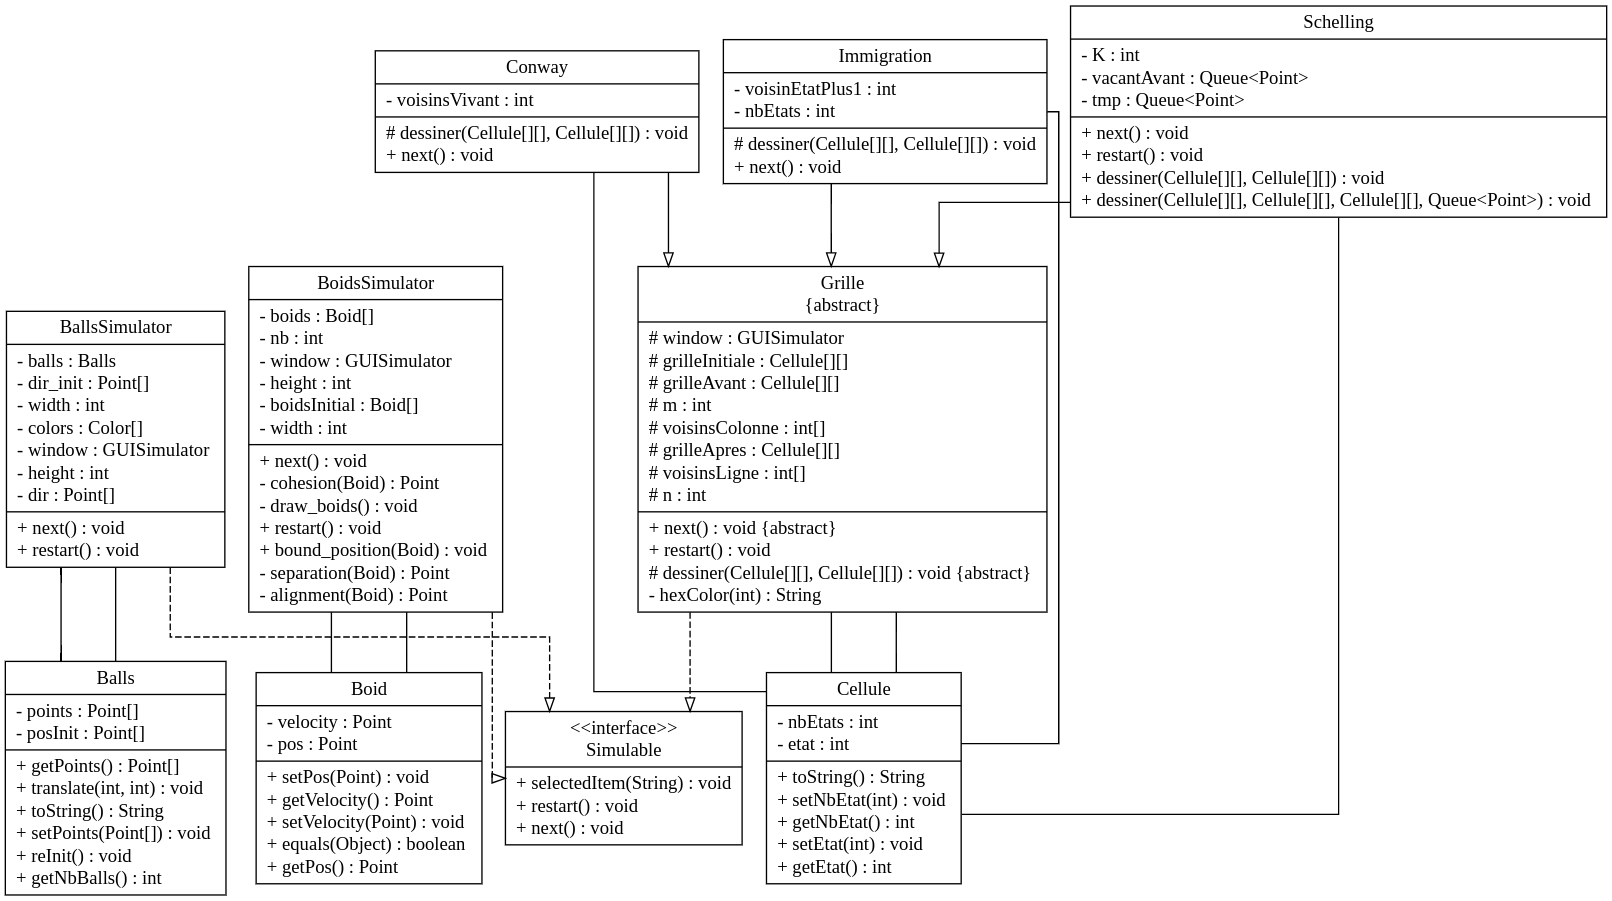
\includegraphics[width=\textwidth]{graph1.png}
    \caption{Diagramme de classes}
    \label{fig:graph1}
\end{figure}

\begin{figure}[H]
    \centering
    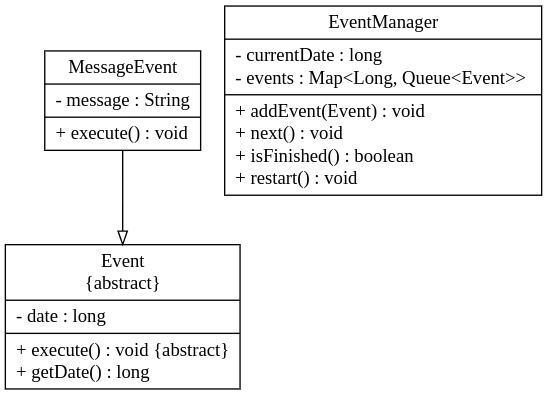
\includegraphics[width=0.4\textwidth]{graph2.png}
    \caption{Diagramme de classes}
    \label{fig:graph2}
\end{figure}

\end{document}